\section{Auswertung}
\label{sec:Auswertung}

\subsection{Bestimmung der Apparatenkonstanten}
Um die Apparatenkonstante zu bestimmen, müssen zunächst die Dichten der Kugeln aus ihren Massen und Radien bestimmt werden. Die zugehörigen Messwerte sind
in \autoref{tab:MasseundDichte} zu finden.

\begin{table}[H]
  \centering
  \caption{Messdaten der Massen und Radien der beiden Kugeln.}
  \label{tab:MasseundDichte}
  \begin{tabular}{c c c c}
    \toprule
    $r_{\text{Gr}}/10^{-2}\,\si{\meter}$ & $m_{\text{Gr}}/10^{-3}\,\si{\kilogram}$ & $r_{\text{Kl}}/10^{-2}\,\si{\meter}$ & $m_{\text{Kl}}/10^{-3}\,\si{\kilogram}$ \\
    \midrule
    1,59 & 4,91 & 1,56 & 4,44 \\
    1,59 & 4,91 & 1,56 & 4,44 \\
    1,59 & 4,91 & 1,57 & 4,44 \\
    1,58 & 4,91 & 1,57 & 4,44 \\
    1,59 & 4,91 & 1,56 & 4,44 \\
    \bottomrule
  \end{tabular}
\end{table}

Die Werte für den Radius und die Masse ergeben sich daraus zu
\begin{align*}
  r_{\text{Gr}} &= (1,588\pm 0,004472) \cdot 10^{-2} \,\si{\meter}, \\
  m_{\text{Gr}} &= (4,91\pm 0,0) \cdot 10^{-3} \,\si{\kilogram}, \\
  r_{\text{Kl}} &= (1,564\pm 0,005477) \cdot 10^{-2} \,\si{\meter}, \\
  m_{\text{Kl}} &= (4,44\pm 0,0) \cdot 10^{-3} \,\si{\kilogram}. \\
\end{align*}

Aus \autoref{eqn:vKugel} folgt somit für die Dichten
\begin{align*}
  \rho_{\text{Gr}} &= (520,38\pm 1,4655) \,\frac{\si{\kg}}{\si{m^3}}, \\
  \rho_{\text{Kl}} &= (492,56\pm 1,7249) \,\frac{\si{\kg}}{\si{m^3}}. \\
\end{align*}

Darüber hinaus werden die Fallzeiten der beiden Kugel im Viskosimeter benötigt. Diese sind für die große Kugel in \autoref{tab:grKugRaum} und für die kleine Kugel
in \autoref{tab:klKugRaum} aufgetragen.

\begin{table}[H]
  \centering
      \caption{Fallzeiten der großen Kugel bei Raumtemperatur ($\SI{20}{\celsius})$.}
      \label{tab:grKugRaum}
      \begin{tabular}{c c}
      \toprule
      Runter $t\:/\:$ s & Hoch $t\:/\:$ s\\
      \midrule
        39,34 & 42,70 \\
        41,82 & 42,02 \\
        42,68 & 41,29 \\
        42,20 & 41,28 \\
        42,16 & 42,38 \\
      \bottomrule
  \end{tabular}
\end{table}

\begin{table}[H]
  \centering
      \caption{Fallzeiten der kleinen Kugel bei Raumtemperatur ($\SI{20}{\celsius})$.}
      \label{tab:klKugRaum}
      \begin{tabular}{c c}
      \toprule
      Runter $t\:/\:$ s & Hoch $t\:/\:$ s\\
      \midrule
        12,87 & 13,13 \\
        12,79 & 13,00 \\
        12,42 & 12,89 \\
        12,66 & 13,02 \\
        12,93 & 12,88 \\
        12,68 & 12,88 \\
        12,80 & 12,69 \\
        12,68 & 13,01 \\
        12,94 & 12,95 \\
        12,29 & 12,94 \\
      \bottomrule
  \end{tabular}
\end{table}

Aus den Messwerten der Fallzeit ergibt sich
\begin{align*}
  t_{\text{Gr}} &= (41,787\pm 0,9910) \,\si{\second}, \\
  t_{\text{Kl}} &= (12,823\pm 0,2053) \,\si{\second}. \\
\end{align*}

Anschließend kann mit Hilfe der Fallzeiten und der angegebenen Konstante der kleinen Kugel $K_{\text{Kl}}$ die Viskosität von Wasser bestimmt werden. Dabei werden
\begin{align*}
  K_{\text{Kl}} &= 7,64\cdot 10^{-8} \,\frac{\si{\pascal}\cdot\si{\meter^3}}{\si{\kilogram}} \\
  \rho_{\text{Fl}} &= 998,2\,\frac{\si{\kilogram}}{\si{\meter^3}} \\
\end{align*}

verwendet, wobei $\rho_{\text{Fl}}$ die Dichte von Wasser bei Raumtemperatur ist. Daraus folgt für die Viskosität bei Raumtemperatur
\begin{align*}
  \eta_{\text{RT}} &= (0,495\pm 0,004052 ) \cdot 10^{-3} \,\si{\pascal}\cdot\si{\second}.
\end{align*}

Daraus ergibt sich mit Hilfe der umgestellten \autoref{eqn:visko} für die Konstante der großen Kugel
\begin{align*}
  K_{\text{Gr}} &= (2,481\pm 0,03982) \cdot 10^{-8} \,\frac{\si{\pascal}\cdot\si{\meter^3}}{\si{\kilo\gram}}
\end{align*}



\subsection{Temperaturabhängigkeit der Viskosität}
Mit Hilfe der Apparatenkonstanten der großen Kugel $K_{\text{Gr}}$ kann nun durch \autoref{eqn:visko} die Viskosität des Wassers bei verschiedenen Temperaturen berechnet werden.
Die Messwerte der Fallzeit der großen Kugel und die verschiedenen Temperaturen mit jeweils zugehöriger Dichte von Wasser sind in \autoref{tab:Temp} dargestellt.

\begin{table}[H]
  \centering
  \caption{Messdaten zur Bestimmung der Temperaturabhängigkeit der Viskosität.}
  \label{tab:Temp}
  \begin{tabular}{c c c c}
    \toprule
    $T/\si{\kelvin}$ & $t/\si{\second}$ & $\rho_{\text{Fl}}/\frac{\si{\kilogram}}{\si{\meter^3}}$ & $\eta/10^{-3}\si{\pascal}\cdot \si{\second}$\\
    \midrule
    296 & 36,84 & 997,54 & 0,436 \\
    299 & 35,24 & 996,79 & 0,417 \\
    302 & 32,70 & 995,95 & 0,386 \\
    305 & 31,02 & 995,03 & 0,365 \\
    308 & 29,25 & 994,03 & 0,344 \\
    311 & 27,91 & 992,97 & 0,327 \\
    314 & 26,28 & 991,83 & 0,307 \\
    317 & 25,23 & 990,63 & 0,294 \\
    320 & 23,89 & 989,37 & 0,278 \\
    323 & 22,66 & 988,04 & 0,263 \\
    \bottomrule
  \end{tabular}
\end{table}

Die Konstanten A und B aus der Andradeschen Gleichung \ref{eqn:andradescheGl} lassen sich durch Auftragen von $ln(\eta)$ gegen $\frac{1}{T}$ in \autoref{fig:plot} und einer
linearen Regression bestimmen.
\begin{align*}
  \eta(T) &= A \, \exp{\left(\frac{B}{T}\right)} \\
  \iff ln(\eta) &= ln(A) + ln(\frac{B}{T}) \\
\end{align*}

\begin{figure}[H]
  \centering
  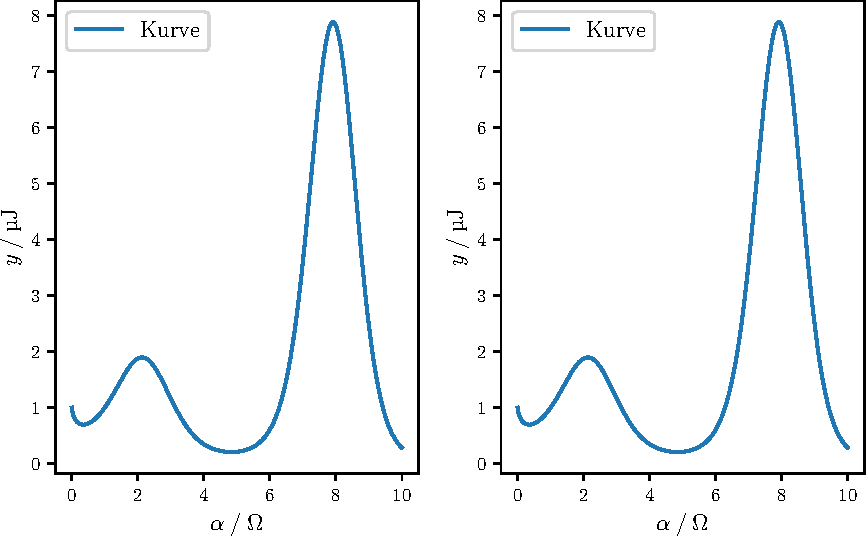
\includegraphics{plot.pdf}
  \caption{Ausgleichsgerade zur Bestimmung der Konstanten der Andradeschen Gleichung.}
  \label{fig:plot}
\end{figure}

Mit Hilfe der linearen Regression ergibt sich
\begin{align*}
  A &= (1801,0960\pm 21,0240) \,\si{\pascal}\cdot\si{\second}\\
  B &= (-9,214\pm 0,0680) \,\si{\kelvin}
\end{align*}

Zuletzt muss geprüft werden, ob es sich im Viskosimeter um eine laminare oder eine turbolente Strömung handelt. Dies passiert, indem die Reynoldszahl für die große und die
kleine Kugel bestimmt und anschließend mit der kritischen Reynoldszahl verglichen wird. Durch \autoref{eqn:reynold} erhält man die Reynoldszahlen
\begin{align*}
  Re_{\text{Gr}} &= 153,26\pm 2,8271\\
  Re_{\text{Kl}} &= 492,03\pm 5,3794.
\end{align*}
Beide Reynoldszahlen liegen unter der kritischen Reynoldszahl von ca. 2300. Es handelt sich demnach um laminare Strömungen.
